\documentclass[a4paper,12pt,french]{article}

\usepackage[cours]{../../../Style}

%\usepackage[theorems]{tcolorbox}

%\newtcbtheorem
%{defi}{Définition}
%{colback=red!5,colframe=red!60!black!80,fonttitle=
%\sffamily\bfseries}{th}

% Début du document
%%%%%%%%%%%%%%%%%%%
\begin{document}

\title{Suites arithmétiques et géométriques}
\maketitle

\begin{programme}
\item représentations graphiques des fonctions : $x \mapsto ax^2,x \mapsto ax^2+b, x \mapsto a(x-x_1)(x-x_2)$
\item axes de symétrie ;
\item racines et signe d'un polynôme de degré 2 donné sous forme factorisée (le calcul des
racines à l'aide du discriminant ne figure pas au programme).
\item Compétences
\begin{itemize}
\item Associer une parabole à une expression algébrique de degré 2
\item Déterminer des éléments caractéristiques de la fonction $x \mapsto a(x-x_1)(x-x_2)$: Signe, extremum, allure, axes de symétrie
\item Vérifier qu'une valeur conjecturée est racine d'un polynôme de degré 2
\item Savoir factoriser dans des cas simples une expression du second degré connaissant une racine.
\item Utiliser la forme factorisée d'un poly pour trouver ses racines et étudier son signe.
\end{itemize}
\item déterminer le signe d'une expression factorisée du second degré
\item résoudre une équation ou une inéquation du premier degré, une équation du type $x^2=a$ avec $a \geq 0$.
\end{programme}

\section{Suites arithmétiques}

\subsection{Généralités}

\begin{defin}
Un premier terme, un nombre r appelé raison et la relation $a_{n+1}=a_n+r$. 

Mettre schéma bulles
\end{defin}

\begin{rmq}
On passe d'un terme au suivant en ajoutant toujours le même nombre. La différence entre deux termes successifs vaut toujours $r$: $a_{n+1}-a_n=r$.

\begin{center}
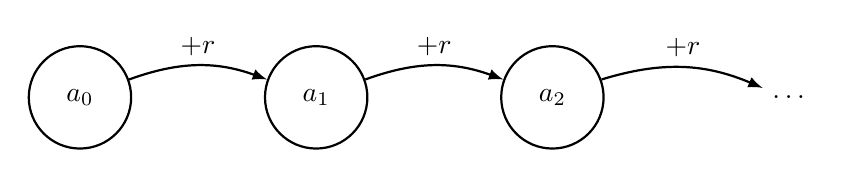
\begin{tikzpicture}[scale=1]
\node[draw,circle,thick, minimum size=13mm] (W0) at (-3,0) {$a_0$};
\node[draw,circle,thick, minimum size=13mm] (W1) at (0,0) {$a_1$};
\node[draw,circle,thick, minimum size=13mm] (W2) at (3,0) {$a_2$};
\node (W5) at (6,0) {$\ldots$};
\draw[->,>=latex,thick] (W0) to[bend left=20] node[midway,above]{$+r$} (W1);
\draw[->,>=latex,thick] (W1) to[bend left=20] node[midway,above]{$+r$} (W2);
\draw[->,>=latex,thick] (W2) to[bend left=20] node[midway,above]{$+r$} (W5);
\end{tikzpicture}
\end{center}

\end{rmq}

\begin{ex}
Soit $u$ la suite arithmétique de premier terme $u_0=5$ et de raison $r=-2$. Alors:
$$
\begin{aligned}
u_1&=u_0-2=3\\
u_2&=u_1-2=1\\
u_3&=u_2-2=-1\\
u_4&=\ \ldots
\end{aligned}
$$
\end{ex}

\begin{rmq}
Points alignés
\end{rmq}

\begin{methode}
Pour s'assurer qu'une suite \textbf{semble} arithmétique, on calcule la différence entre deux termes successifs, et l'on doit toujours trouver le même nombre (la raison).
\end{methode}

\begin{ex}
Tableau de valeurs pour deux suites. L'une parait arithmétique, l'autre non.
\end{ex}

\subsection{Variations des suites arithmétiques}

\begin{prop}
\begin{itemize}
\item Si $r > 0$, alors la suite $a$ est croissante.
\item Si $r < 0$, alors la suite $a$ est décroissante.
\item Si $r = 0$, alors la suite $a$ est constante.
\end{itemize}
\end{prop}

\begin{ex}
..
\end{ex}

\section{Suites géométriques, cas positif}

\subsection{Généralités}

\begin{defin}
Un premier terme, un nombre $q$ appelé raison et la relation de récurrence $g_{n+1}=q \times g_n$.

Mettre schéma bulles
\end{defin}

\begin{rmq}
On passe d'un terme au suivant en multipliant toujours par le même nombre. Le quotient de deux termes successifs vaut toujours $q$: $\frac{g_{n+1}}{g_n}=q$.
\end{rmq}

\begin{ex}
ex
\end{ex}

\subsection{Variations des suites géométriques}

\begin{prop}
\begin{itemize}
\item Si $q > 1$, alors la suite $g$ est croissante.
\item Si $0< q < 1$, alors la suite $g$ est décroissante.
\item Si $q = 1$, alors la suite $g$ est constante.
\end{itemize}
\end{prop}

\begin{ex}

\end{ex}

\begin{deroule}
\item \textbf{Total: 3.5 semaines}
\item Semaine 1
\begin{itemize} 
\item 30m - Cours I partie 1: Définitions et exo
\item 15m - Graphe de $x \mapsto x^2$
\item 1h - Cours: Représentation graphique, sommet, variations, exo
\item 30m - Cours II: Généralités+Exos
\end{itemize}
\item Semaine 2
\begin{itemize}
\item 1h - Suite
\item 1h - II.2 + Exos
\item 45m - III.1.1 + Exos
\item 45m - III.1.2 + Exos
\end{itemize}
\item Semaine 3
\begin{itemize}
\item 30m - Suite
\item 45m: III.1.3 + Exos
\item 1h: III.2 + Exos
\item 1h: III.3 + Exos
\end{itemize}
\end{deroule}

\end{document}
